\documentclass[11pt]{article}
\usepackage[margin=1.2in]{geometry}
\usepackage{graphicx}
\usepackage{fancyhdr}
\usepackage{nopageno}%removes number on titlepage
\usepackage[parfill]{parskip}%adds lines in between paragraphs and takes out indentation
%\usepackage{subfig}
%\usepackage{multirow}
\usepackage{caption}
\usepackage{subcaption}

\begin{document}
% Cover page
\author{Chelsey Legacy, Lindong Zhou, Evan Pete Walsh\footnote{Statistics graduate students at Iowa State University of Science and Technology}}
\title{Visualizing Factors that Make Bars, Restaurants, and Hotels Popular}
\maketitle

\begin{abstract}
Blah blah blah
\end{abstract}

\newpage

\tableofcontents

\newpage

\pagenumbering{arabic}%starts numbering at "1"
\pagestyle{fancy}
\fancyhead[L]{Iowa State University}
\rhead{\thepage}
\rfoot{\today}
\cfoot{}%removes default page number at bottom center


\section{Introduction}

The Yelp Academic Dataset\footnote{$https://www.yelp.com/academic\_dataset$} provides data enthusiants with the exciting opportunity to explore an incredible collection of information regarding the characteristics and quality of hundreds of businesses across the United States, Canada, and the UK. This paper provides some thorough insight into the data using a variety of visualization techniques. 

In particular, we investigate various factors that affect the rating of restaurants, bars, hotels, and shopping centers. For restaurants, we seek to answer how whether or not an establishment accepts reservations influences the price and the overall quality of the dining experience. We also investigate how noise level effects the rating of restaurants and how this differs between places that offer live music and those that do not. Lastly, we use a pair of wordclouds to question the types of things people are most likely to talk about when they write a ``tip"\footnote{In Yelp, a ``tip" is a short comment or description of a business given by a Yelp user. A tip is too short to be considered a review.} about a really bad or really fantastic restaurant.

For bars,

For hotels and shopping, 

This paper will procede as follows: Section 2 discusses the raw data and the steps that were taken to ``clean" the data into a more useful form. Section 3 examines the subset of data associated with restaurants, while sections 4, 5, and 6 examine the subsets associated with bars, hotels, and shopping, respectively. We conclude in section 7 by summarizing what we have found and offering several ideas for future studies.


\section{Data}

The Yelp Academic Dataset\footnote{$https://www.yelp.com/academic\_dataset$} provides data enthusiants with the exciting opportunity to explore an incredible collection of information regarding the characteristics and quality of hundreds of businesses across the United States, Canada, and the UK. Specifically, the data includes details and reviews on 250 of the closest businesses to 30 large universities, including the Arizona State, UNLV, the University of Edinburgh, the University of Wisconsin, and the University of Waterloo, to name a few. The raw data is in json format and contains five different types of json objects: \textbf{Business}, \textbf{Review}, \textbf{User}, \textbf{Check-in}, and \textbf{Tip}.

Each \textbf{Review} object represents an individual user-based review of a particular business. The unique encrypted business ID is given along with the date of the review, the number of stars (out of 5) that were awarded, the number and type of votes that the review received, and an optional text description provided by the user. \textbf{User} objects are unique to every person that has an active Yelp account. Each user has a name, a unique encrypted user ID, the number of votes they have cast, the average number of stars they have given, and the date they signed up for Yelp, among other things. A \textbf{Check-in} object represents the count and time of all the registered check-ins for a particular business, and \textbf{Tip} objects represent a tip given by user for a particular business. Tips include the user's ID, the business's ID, the date, and the message that the user gave. While these objects all provide a rich source of information, for the scope of this paper we will only be examing the \textbf{Business} objects.

\textbf{Business} objects are unique to business ID's, and include the following information:
\begin{itemize}
	\item the name of the business,
	\item the name of neighborhood in which the business is located,
	\item the city in which the business is located,
	\item the full address of the business,
	\item the exact latidude and longitude coordinates of the business,
	\item the average number of stars awarded to the business,
	\item the number of reviews received by the business,
	\item whether or not the business is still open,
	\item the hours that the business is open,
	\item the categories that the business falls under,
	\item and a number of different attributes which mostly concern restaurants and bars, such as whether or not smoking is allowed and the price range of the food.
\end{itemize}

To work with the data, we converted the set of all \textbf{Business} objects to a csv file in which the columns are variable names representing each aspect of a \textbf{Business} object, and each row corresponds to a unique business. Each different type of attribute was converted to its own character, numerical, or logical variable depending on what was appropriate. For example, the attribute \textbf{smoking} was converted to a logical variable where the value is ``true" if the smoking is allowed at the establishment, and ``false" if it is not allowed, while the attribute \textbf{price range} was converted to a numerical variable which ranges from 1 to 4.



\section{Restaurants}

Most of the data about restaurants in the Yelp Academic Dataset are concentrated around the following cities:
\begin{itemize}
	\item Madison, WI, 
	\item Las Vegas, NV,
	\item Pheonix, AZ,
	\item Waterloo, Ontario, Canada,
	\item and Edinburgh, Scotland.
\end{itemize}
Although the choice of cities is limited, the wealth of information coming from each city is abundant. All together, our data consists of 14,303 restaurants with 45 variables describing their attributes and the collective user sentiment towards each establishment. There is a significant number of restaurants in just about any subcategory that one can imagine. For example, Figure~\ref{fig:food01a} shows all of the restaurants classified as either ``hipster" or ``divey" near Pheonix, AZ that have televisions, offer live music, and have more than 35 reviews on Yelp. Figure~\ref{fig:food01b} shows all of the Asian and Indian food restaurants near Las Vegas, NV that offer take-out and have a full bar.

\begin{figure}[h]
\caption{Restaurant subsets near Pheonix, AZ and Las Vegas, NV.\label{fig:food01}}
\centering
\begin{subfigure}{0.45\linewidth}
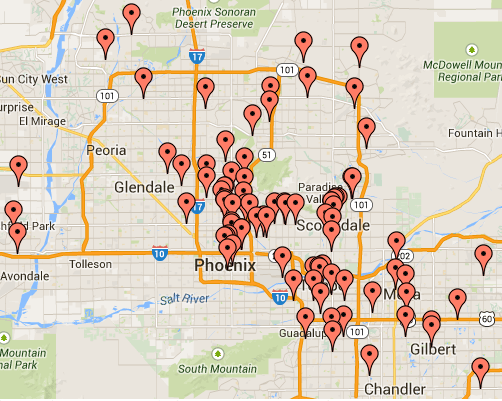
\includegraphics[width=\linewidth]{Figures/food_AZ.png}
\caption{\footnotesize{All restaurants near Pheonix, AZ classified as ``hipster" or ``divey" that have live music, TV's, and more than 35 reviews on Yelp.}}
\label{fig:food01a}
\end{subfigure}
\begin{subfigure}{0.45\linewidth}
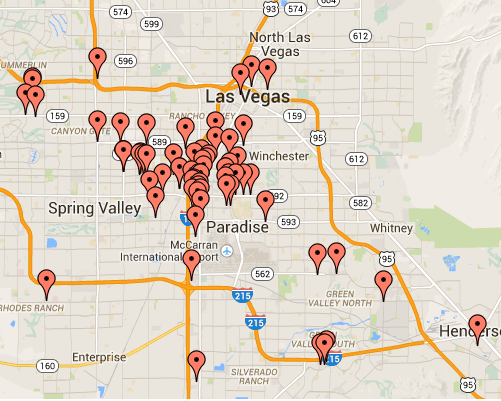
\includegraphics[width=\linewidth]{Figures/food_NV.png}
\caption{\footnotesize{All Asian and Indian food restaurants near Las Vegas, NV that offer take-out and have a full bar.}}
\label{fig:food01b}
\end{subfigure}
\end{figure}

\subsection{The Cost of Reservations}

One question we have explored with the data is whether restaurants that take reservations are more expensive and of higher quality than those that do not. Not suprisingly, it appears that one has to pay a premium, on average, to eat out at a restaurant that accepts reservations. Figure~\ref{fig:food_res_price} shows the average price level of restaurants by type that do or do not accept reservations. For each category, the price level is higher on average for restaurants that accept reservations.

There are a couple potential explanations for this. For one, it could just be that fancier restaurants feel they need to accept reservations to attract their target demographic. Perhaps people who are willing to spend a large amount on a meal will only do so if they know they will be seated right when they arrive. Or maybe restaurants that take reservations lose some money in transition time when open tables are kept unoccupied until the party that made the reservation arrives. The higher average price of restaurants that take reservations could just be making up for this inefficiency.

\begin{figure}[h]
\caption{Price scale of restaurants by type and whether they accept reservations.}
\centering
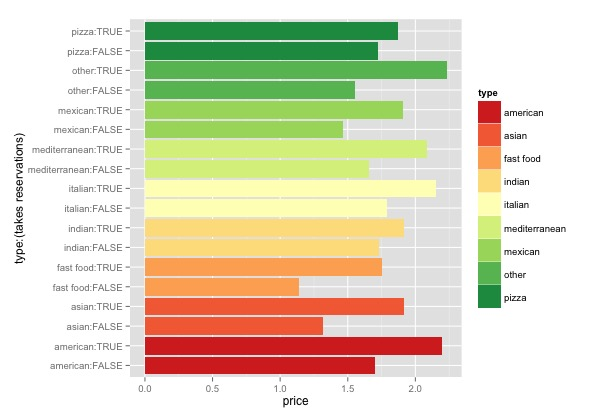
\includegraphics[width=0.7\linewidth]{Figures/food_res_price.jpeg}
\label{fig:food_res_price}
\end{figure}

Although a premium is payed to eat at restaurants that accept reservations, we find that the quality of the experience does not necessarily increase, as measured by the average stars awarded by Yelp users. Figure~\ref{fig:food_res_stars} compares the average stars received by each category by whether or not reservations are accepted. While the average number of stars is slightly higher for pizza, fast food, Asian, American, and ``other" style restaurants that take reservations, the average star count is actually lower for Mexican, Mediterranean, Italian, and Indian style restaurants.

\begin{figure}[h]
\caption{Rating of restaurants by type and whether they accept reservations.}
\centering
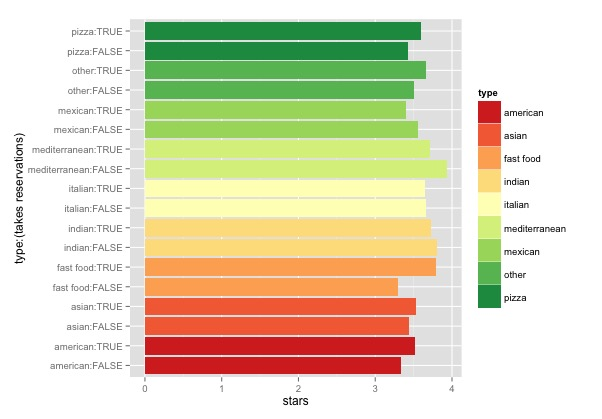
\includegraphics[width=0.7\linewidth]{Figures/food_res_stars.jpeg}
\label{fig:food_res_stars}
\end{figure}

The reason for this discrepancy is unclear. Maybe popular restaurants in certain categories just don't accept reservation because it would be too inefficient, and customers are fine with that. Price may also have something to do with it. Figure~\ref{fig:food_res_3} shows the rating of restaurants by type, whether they accept reservations, and price level. For Mexican restaurants, the average rating of low priced establishments is indistinguishable between those that accept reservations and those that do not. Yet for those in the third price level, the rating is clearly higher for those that do not take reservations. The same is true for Asian style restaurants while the opposite holds for Italian and American style restaurants. This could be because people who generally like to eat at pricier Italian and American food restaurants prefer to be able to make reservations, so these restaurants that allow reservations end up with higher ratings.

\begin{figure}[p]
\caption{Rating of restaurants by type, whether they accept reservations, and price level.}
\centering
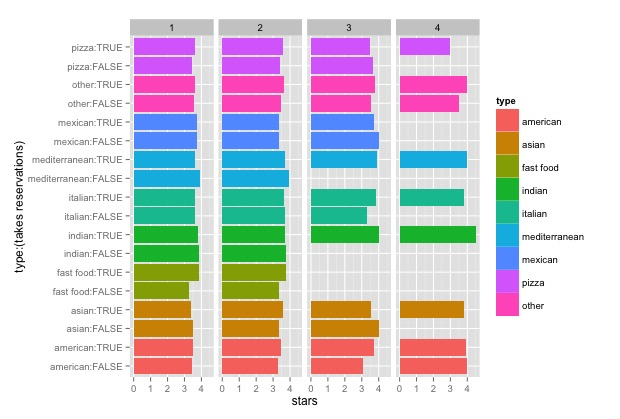
\includegraphics[width=0.8\linewidth]{Figures/food_res_3.jpeg}
\label{fig:food_res_3}
\end{figure}

\subsection{Loud can be Good, but not too Loud}

Another question we sought to answer was how noise pollution affects the quality of a dining experience, especially when we consider whether or not the establishment offers live music. One can imagine that people deliberately going out to eat at a restaurant with a band playing might bear a higher noise level, and thus not be as quick to penalize the restaurant for being too noisy in their review. We find that the data is consistent with this hypothesis.

For restaurants that offer live music, as shown in Figure~\ref{fig:food_noise}, loud places have a higher average rating than places with an average noise level. Yet very loud places have the lowest average rating. For restaurants that do not offer live music, the average rating decreases with the noise level.

\begin{figure}[p]
\caption{Rating of restaurants by their noise level and whether they host live music. The plot on the left shows the rating of restaurants by noise level that do not have live music, and the plot on the right shows the rating for restaurants with live music.}
\centering
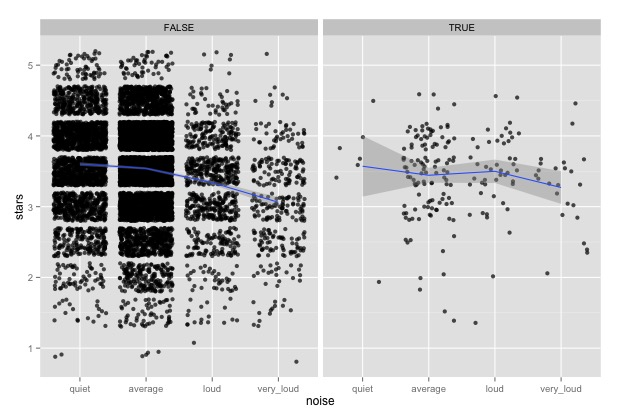
\includegraphics[width=0.7\linewidth]{Figures/food_noise.jpeg}
\label{fig:food_noise}
\end{figure}


\subsection{It's All About Service}

It will come as no surprise that service is a vital part of the service industry. Friendly, competent staff can make or break the dining experience. To illustrate the validity of this statement, we examined the \textbf{Tips} objects to see which words came up the most when Yelp users were describing either a really bad or really good restaurant experience. We first matched every single restaurant tip with the corresponding restaurant, and then sorted the tips by the average number of stars that each restaurant has. We then used a simple visualization technique on each set, called a wordcloud. 

A wordcloud is formed by displaying the most frequently occuring words from a set together in a random, or partly random, arrangement. The size of each word is weighted by how many times it appears in the set. A coloring scheme is often added to complemented the size weighting.

We first took a random sample of 600 tips corresponding to restaurants with at least 4.5 stars, and 600 corresponding to restaurants with less than 2 stars. We then created a wordcloud for each set of tips after removing certain words like ``great," ``awesome," and ``love" from the high rating group and words like ``bad," ``terrible," and ``don't" from the low rating group, because those words are obvious and appeared so frequently that they ``clouded" out more interesting words. There were also other words like ``try," ``place," and ``get" that were removed from both groups for the same reasons. The resulting wordclouds are shown in Figures~\ref{fig:wordcloud_a}, for the high rating group, and~\ref{fig:wordcloud_b} for the low rating group.

\begin{figure}[h]
\caption{Wordclouds of tips for great restaurants and terrible restaurants.\label{fig:wordcloud}}
\centering
\begin{subfigure}{0.49\linewidth}
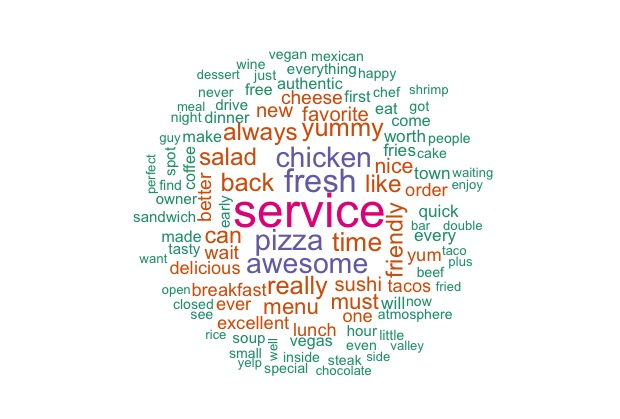
\includegraphics[width=\linewidth]{Figures/wordcloud_top.jpeg}
\caption{\footnotesize{Tips for restaurants with atleast 4.5 stars.}}
\label{fig:wordcloud_a}
\end{subfigure}
\begin{subfigure}{0.49\linewidth}
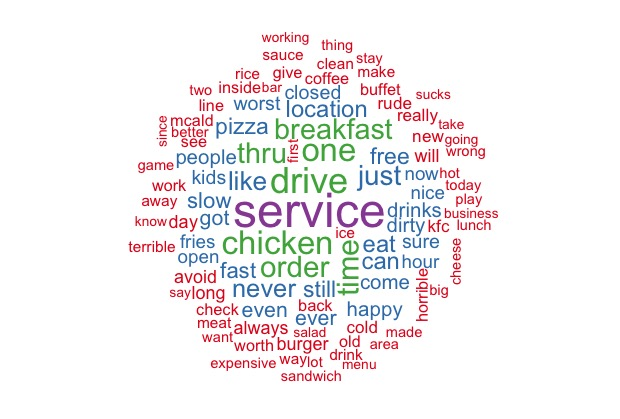
\includegraphics[width=\linewidth]{Figures/wordcloud_bottom.jpeg}
\caption{\footnotesize{Tips for restaurants with less than 2 stars.}}
\label{fig:wordcloud_b}
\end{subfigure}
\end{figure}

The interesting thing to notice here is that both wordclouds look extremely similar. Words like ``chicken," ``pizza," ``time," and ``order" are found in each set. Further, in both cases the word ``service" was the most frequent word. Thus, it seems that people with either really good or really bad experiences tend to comment on the same types of things, particularly when it comes to service.



\section{Bars}

Chelsey

\section{Hotels}

Lindong


\section{Conclusion}


Chelsey




\end{document}